\newpage
\section{Projections}
\begin{figure}[H]
  \centering
  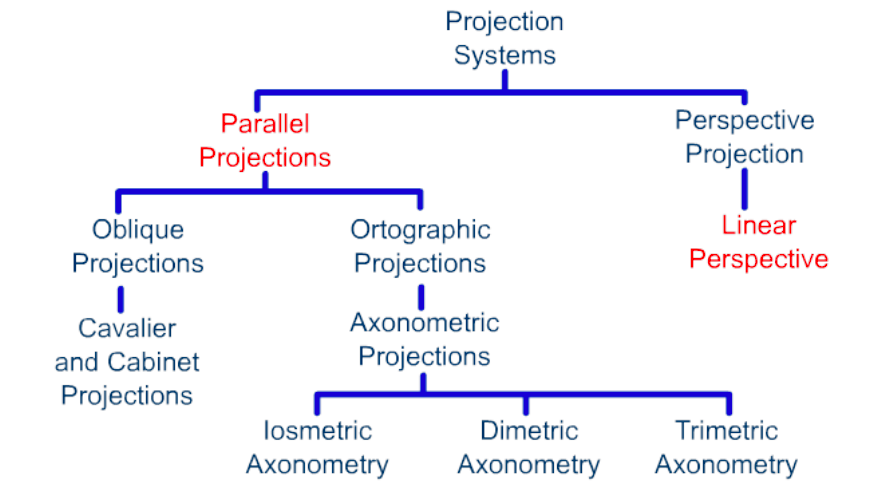
\includegraphics[width=.6\linewidth]{projections}
\end{figure}
In 3D computer graphics the goal is to represent a three dimensional space on a screen with 2 dimensions:
\begin{itemize}
\item The 3D graphics uses geometrical primitives defined in 3 dimensions
\item 3D graphics produces  a 2D representation of the scene to show on screen.
\end{itemize}
The second step is performed using \textbf{projections}.
Key features :
\begin{itemize}
\item Projections of linear segments \textbf{remain} linear segments 
\item Projected segments connect the projections of the segment's end points
\end{itemize}
So to create a 2D projection of a 3D polyhedron it is sufficient to \textbf{project its vertices} and connect them.\\
In parallel projections all the rays are \textbf{parallel to the same direction}.\\
In perspective projections all the rays pass \textbf{through a point} called \begin{figure}[H]
\begin{minipage}{.5\textwidth}
 \centering
  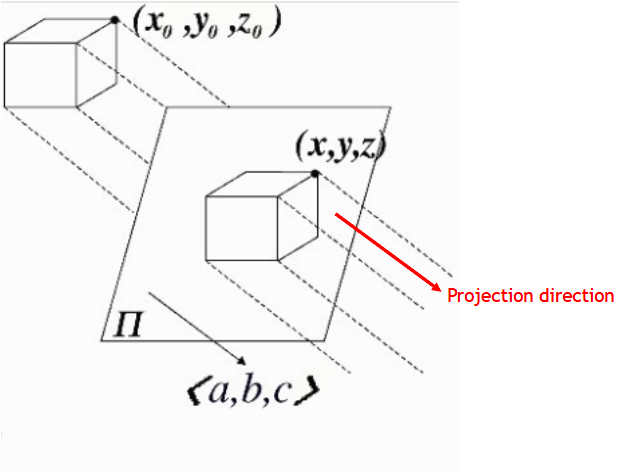
\includegraphics[width=.6\linewidth]{parallel}
\end{minipage}%
	\begin{minipage}{.5\textwidth}
  \centering
  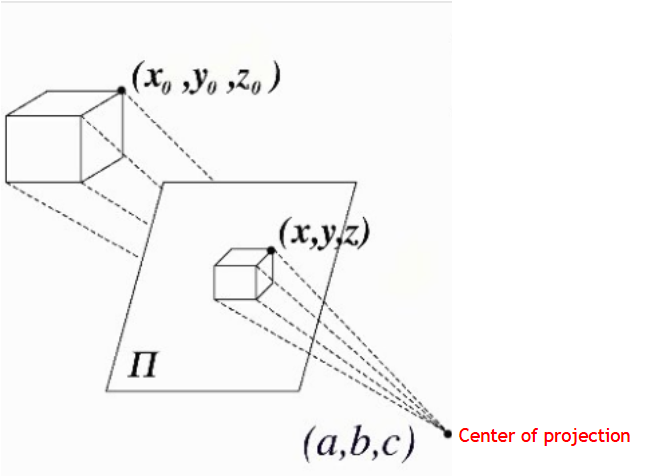
\includegraphics[width=.6\linewidth]{perspective}
\end{minipage}%
\end{figure}
Doing a projection , we loose one coordinate so a point on screen corresponds to an \textbf{infinite} number of coordinates ( consequence of moving from 3D $\to$ 2D) : in both parallel \& perspective projections any point on screen corresponds to \textbf{a line of points} in 3D.
In parallel projections all points that pass	through a line parallel to projections ray are mapped to the \textbf{same pixel}.\\
In perspective projections all points aligned with both projected pixel and the center of projection are mapped to the \textbf{same pixel}.
\begin{figure}[H]
\begin{minipage}{.5\textwidth}
 \centering
  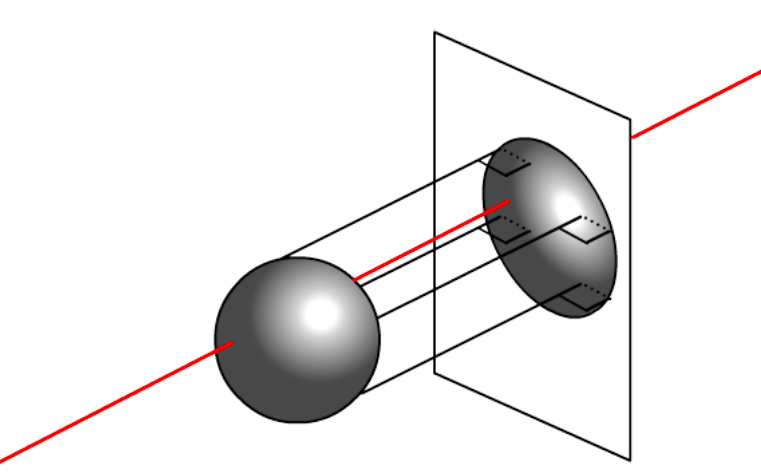
\includegraphics[width=.6\linewidth]{parallel_prop}
\end{minipage}%
	\begin{minipage}{.5\textwidth}
  \centering
  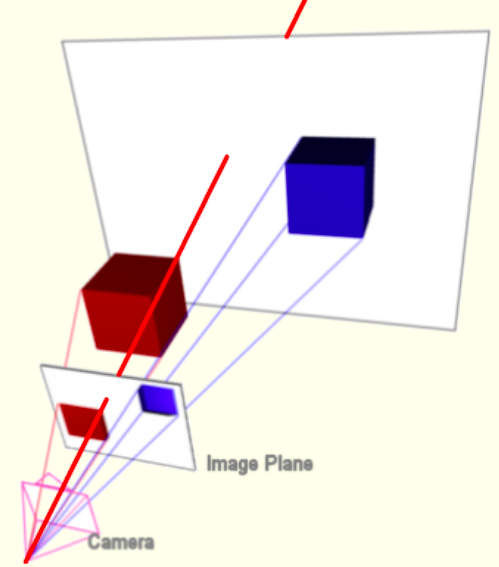
\includegraphics[width=.5\linewidth]{perspective_prop}
\end{minipage}%
\end{figure}
In 3D computer graphics the concept of projection becomes the \textbf{conversion} of 3D coordinates from one reference system to another.\\
\textbf{World coordinates}$\to$ \textbf{3D Normalized Screen Coordinates}\\
\begin{description}
\item[World coordinates]\hfill\\
Coordinate system that describes the objects in the 3D space. It is a right-handed Cartesian coordinate system with the \textbf{origin} in the \textbf{center of the screen.}
Some applications invert the z and y axis , with the y axis point inside the screen.
\begin{figure}[H]
 \centering
  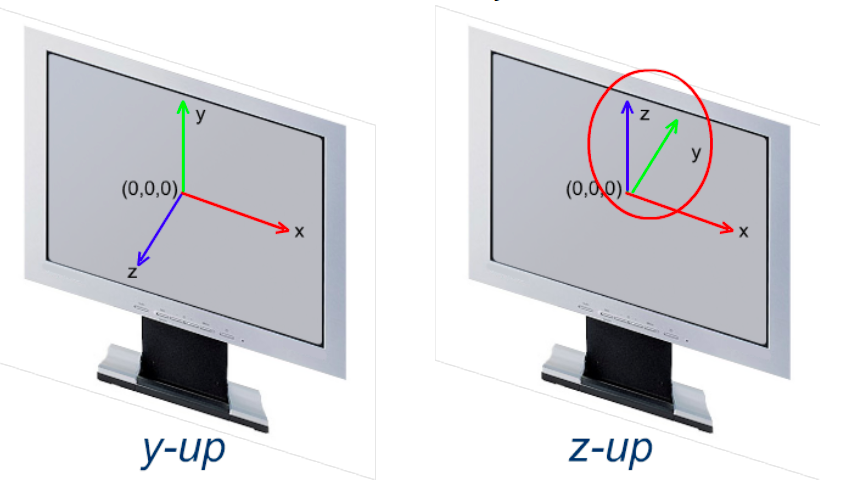
\includegraphics[width=.4\linewidth]{world}
\end{figure}
\item[3D Normalized Screen Coordinates]\hfill\\
Allow to specify the positions of points on screen (or window) in a device-independent way. 3D images must be characterized by a \textbf{distance} to allow ordering the surfaces and prevent the construction of unrealistic images.\\
3D Normalized coordinates have a \textbf{third} component ranging form the same extents (ex : -1,1). This way coordinates with a smaller z-value will be considered to be \textbf{closer} to the viewer.
\begin{figure}[H]
 \centering
  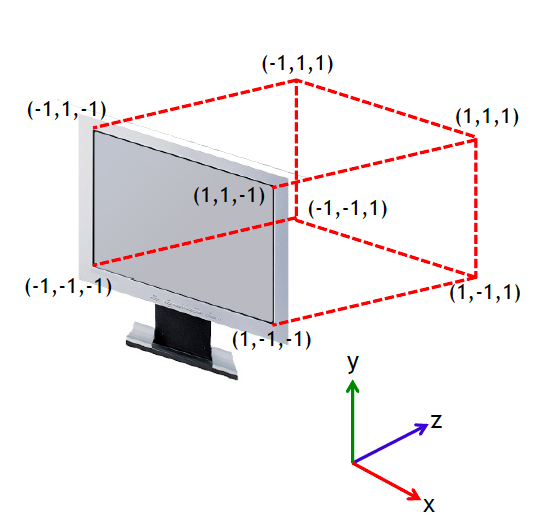
\includegraphics[width=.4\linewidth]{3dnorm}
\end{figure}
\end{description}

\subsection{Parallel Projections}
\textbf{Orthogonal projections} are projections where the plane is either xy,xz or yz and the \textbf{projections rays} are \textbf{perpendicular to it}.
\begin{description}
\item[Projection plane parallel to xy-plane]\hfill\\
The projections are \textbf{perpendicular} to the \textbf{z-axis}.
Limiting the range of a scene is important to avoid showing objects \textbf{behind the observer} or \textbf{too far away} :
\begin{itemize}
\item The plane with the \textbf{minimum z component } $\to$ \textbf{near plane}
\item The plane with the \textbf{maximum z component } $\to$ \textbf{far plane}
\end{itemize}
\begin{figure}[H]
 \centering
  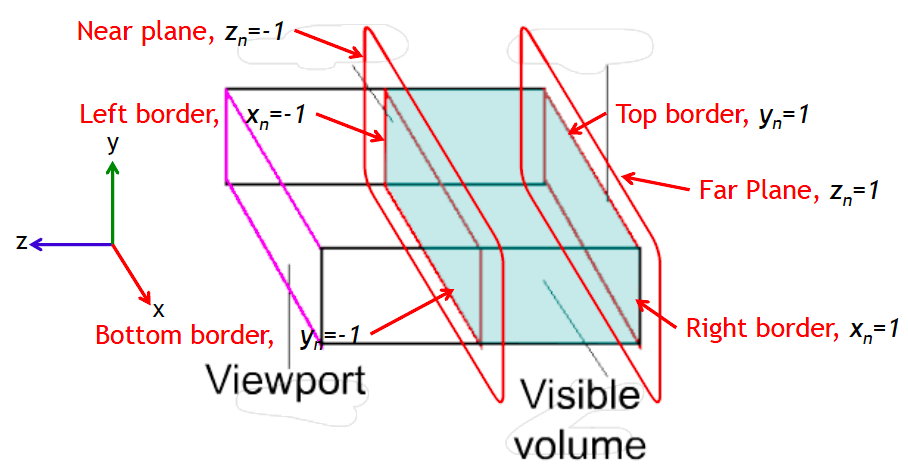
\includegraphics[width=.4\linewidth]{planes}
\end{figure}
Usually distance from viewport to near plane is very small. Things before the near plane and behind the far plane are \textbf{not shown} in the scene: only the visible volume will be seen.\\
\end{description}
\textbf{Orthogonal projections} can be implemented by \textbf{normalizing} the x,y,z coordinates of the projection box in the (-1,1) range. Then a \textbf{projection matrix} can be computed to find the normalized 3D coordinates :
$$ p_N = P_{ort}\cdot p_W$$
How to find $P_{ort} $?\\
Coordinates l,r are the \textbf{x-coordinates} in the 3D space that will be displayed on the left and right borders of the screen. Everything on the left of l or right of r will be \textbf{cut}.\\
Similarly t,b are the \textbf{y-coordinates} of the top and bottom borders of the screen.\\ 
Finally we call -n ,-f the \textbf{z-coordinates} of the near and far planes . Since the z-axis is oriented in the opposite direction the positive distance is used over the negative one. Also using this annotation means that $n>f$ even if n is closer than f!
Bottom left front point will have coordinates (-1,-1,-1) while the top right back point has coordinates (1,1,1).\\
To create the $P_{ort}$ matrix:
\begin{enumerate}
\item Move the center of the box to correspond to the center of the space\\The center of the box will have coordinates :$$ c = ( \frac{l+r}{2}, \frac{t+b}{2}, \frac{f+n}{2})$$
So to align the center we must \textbf{inverse translate} $$ c' = T^{-1}(\frac{l+r}{2}, \frac{t+b}{2}, \frac{f+n}{2}) \cdot c$$ so that the center now corresponds to the origin. 
\begin{figure}[H]
 \centering
  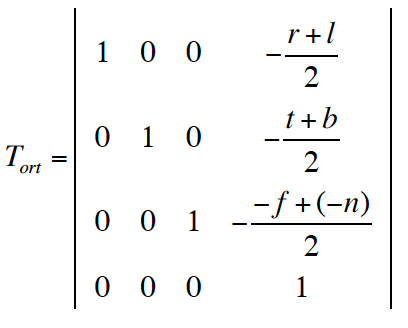
\includegraphics[width=.3\linewidth]{t_ort}
\end{figure}
\item Then normalise the coordinates \\
\begin{figure}[H]
 \centering
  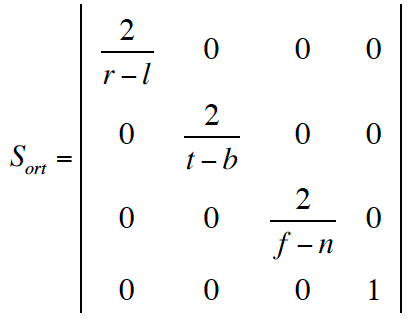
\includegraphics[width=.3\linewidth]{s_ort}
\end{figure}
\item Z goes to the viewer : points closer should have inverse Z coordinate\\
Changing the sign of Z is done by mirroring :
\begin{figure}[H]
 \centering
  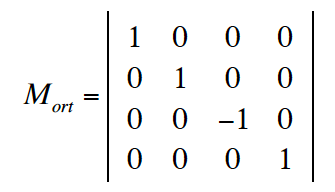
\includegraphics[width=.3\linewidth]{m_ort}
\end{figure}
\end{enumerate}
Which can be resumed by using a single combined matrix:
\begin{figure}[H]
 \centering
  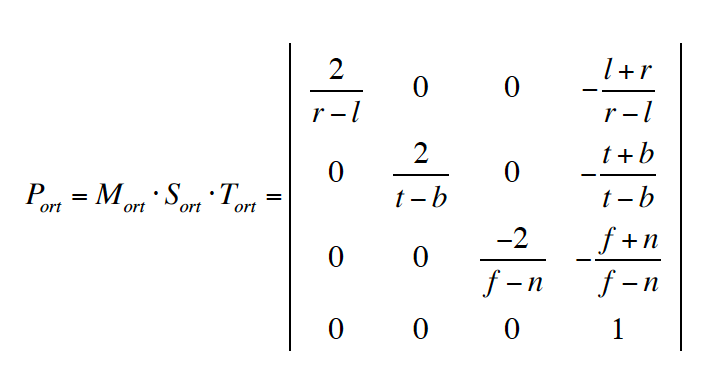
\includegraphics[width=.5\linewidth]{comb_ort}
\end{figure}
